\documentclass[11pt,a4paper]{article}
\usepackage[latin5]{inputenc}
\usepackage[english]{babel}
\usepackage{amsmath}
\usepackage{amsfonts}
\usepackage{amssymb}
\usepackage{graphicx,subfig}
\usepackage{placeins}
\usepackage{gensymb}


\begin{document}

\section*{Report Exercise 5 Advanced Part, Alexander Attinger \& Yannic Kilcher}

\section{RANSAC Matching}
We have used the SURF detector and descriptor to locate interest points in the library and book images.
We then have matched the book images with the library image, as can be seen on Fig. \ref{fig:e1}.
We have then used RANSAC to the best matches using random sampling of 3 matches 10000 times and calculated for each sample an affine transformation.
With the affine transformation, we transferred the book image into the library image and calculated the squared error of the known corresponding points.
We have selected the best affine transformation and subtracted the transformed book image from the library image. The results can be seen on Fig. \ref{fig:e2}.
Our observation is that, the more matches are found, the better the affine transformation can be determined.
\begin{figure}%
\centering
\subfloat[][]{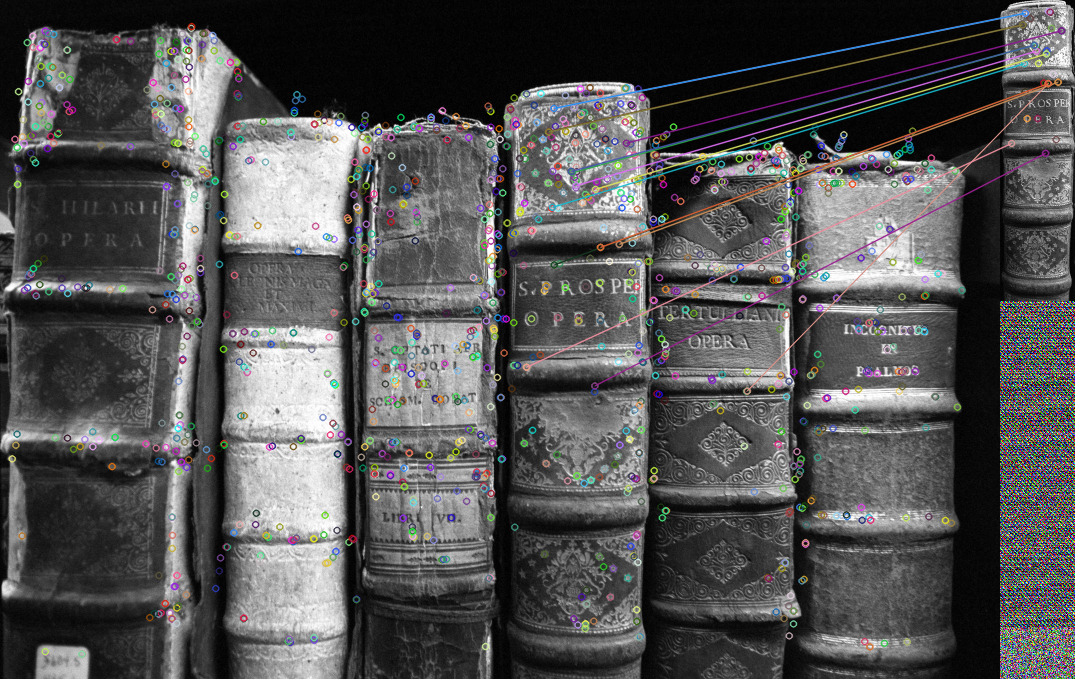
\includegraphics[scale=.2]{data/res/matches_book.png}}
\quad
\subfloat[][]{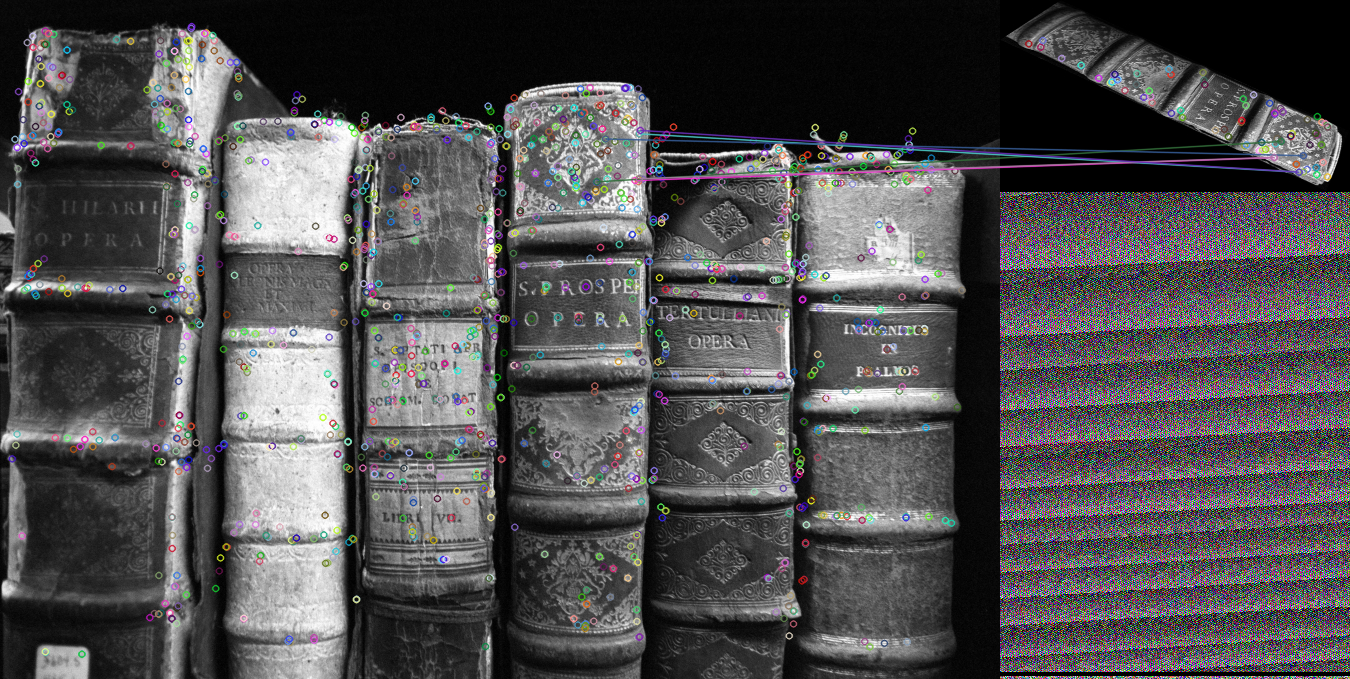
\includegraphics[scale=.2]{data/res/matches_bookP.png}}
\quad
\subfloat[][]{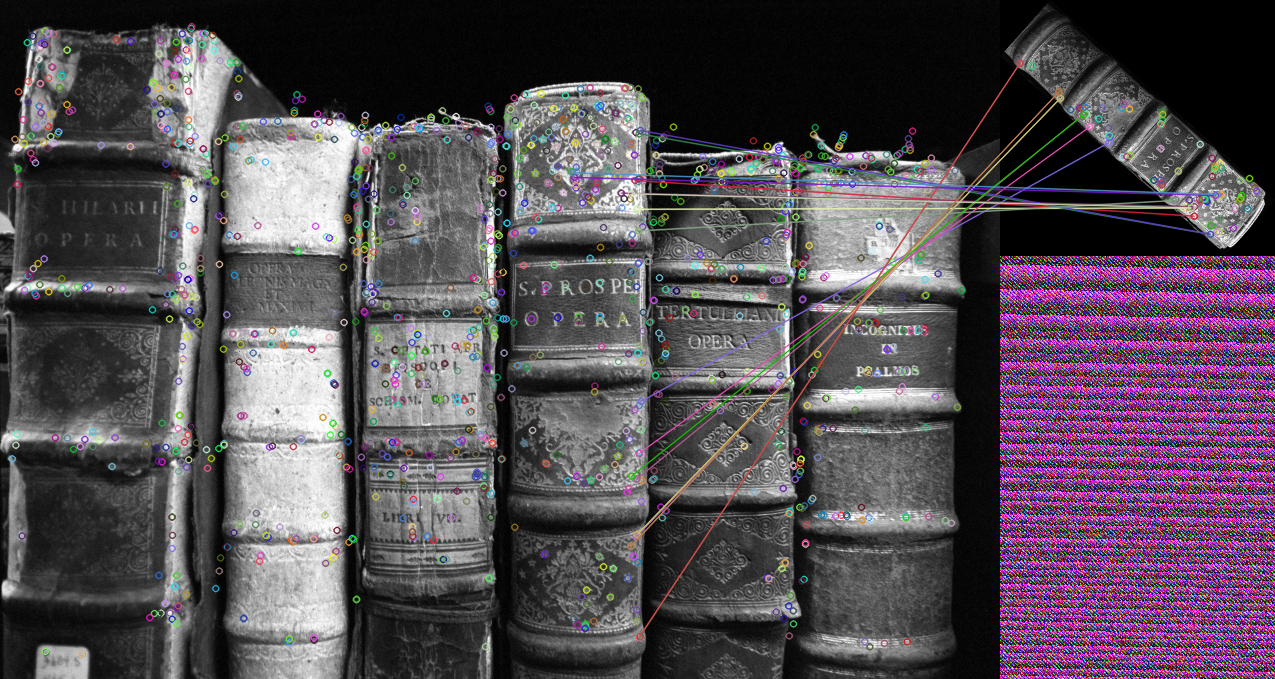
\includegraphics[scale=.2]{data/res/matches_bookR.png}}
\quad
\subfloat[][]{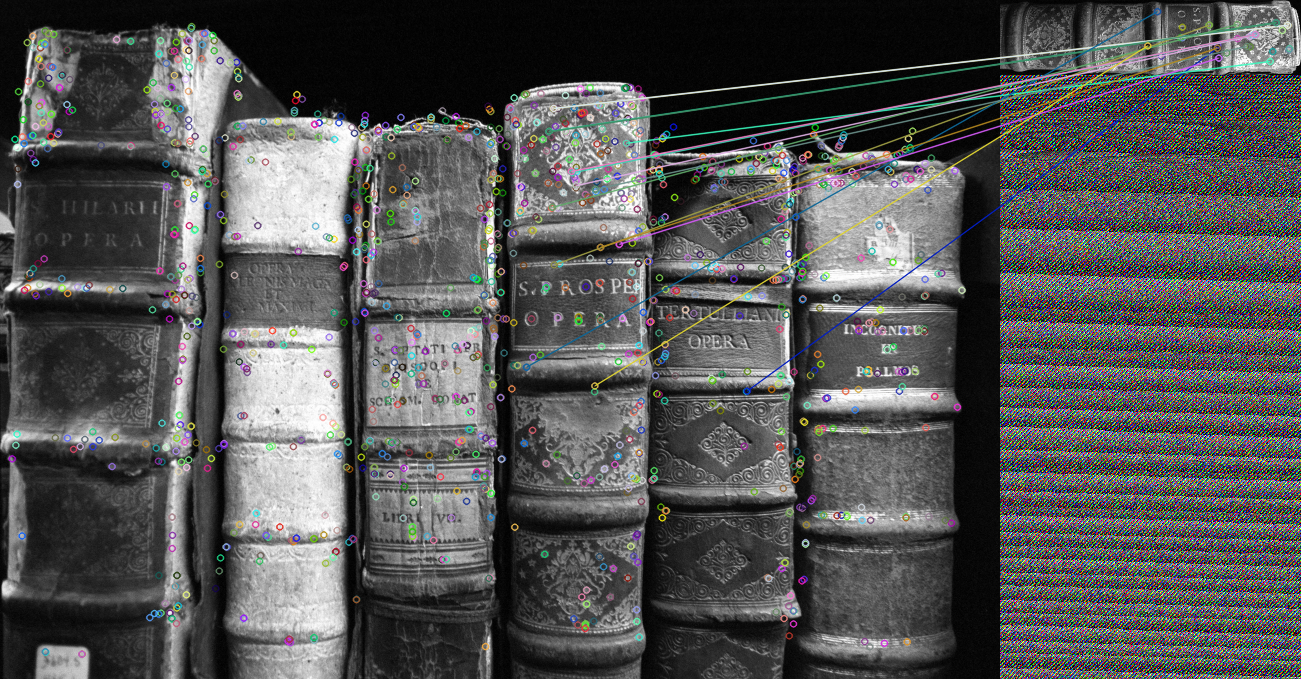
\includegraphics[scale=.2]{data/res/matches_bookT.png}}
\quad
\caption{SURF Matches}%
\label{fig:e1}%
\end{figure}
\begin{figure}%
\centering
\subfloat[][]{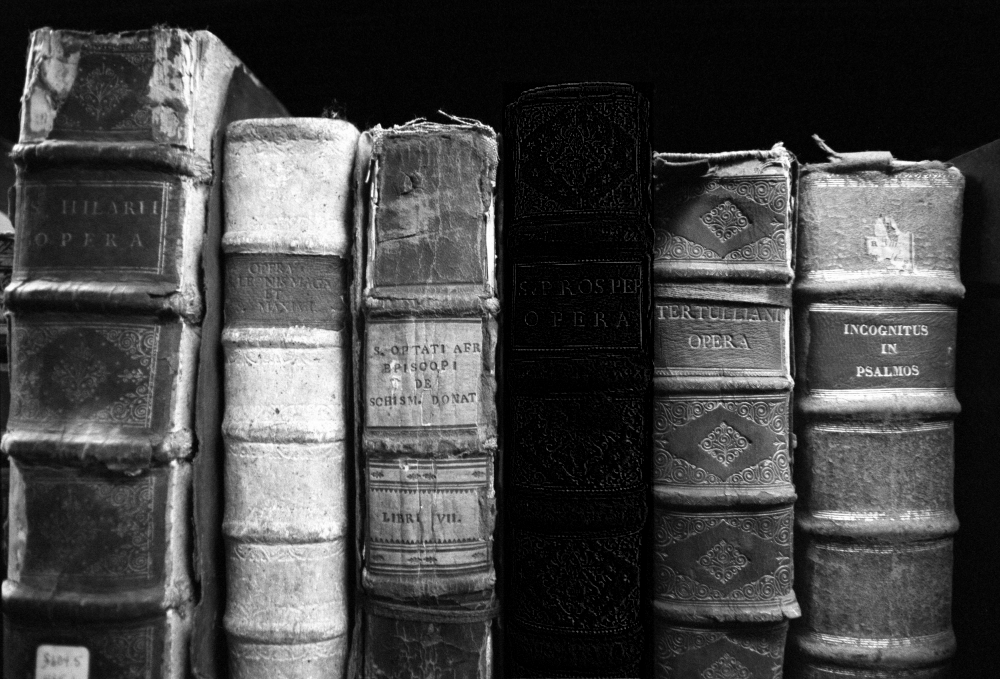
\includegraphics[scale=.2]{data/res/warped_book.png}}
\quad
\subfloat[][]{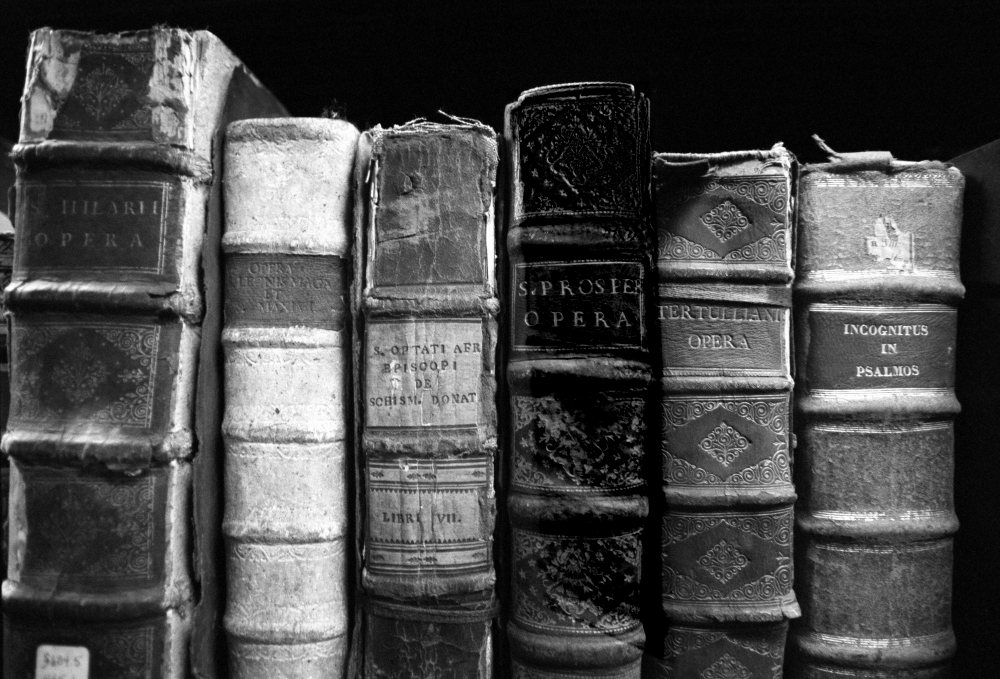
\includegraphics[scale=.2]{data/res/warped_bookP.png}}
\quad
\subfloat[][]{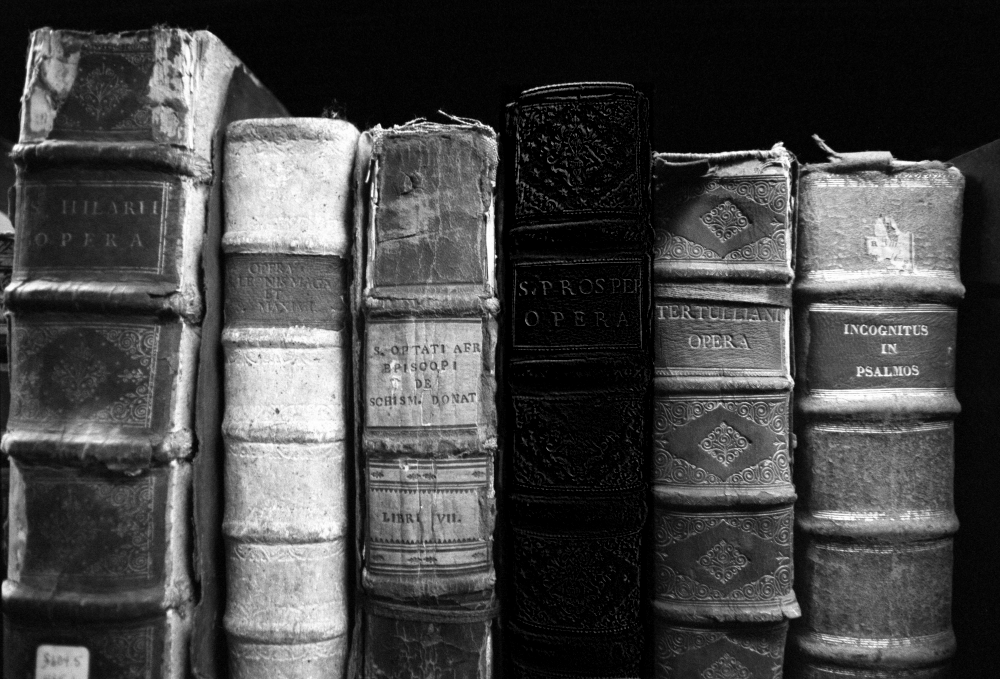
\includegraphics[scale=.2]{data/res/warped_bookR.png}}
\quad
\subfloat[][]{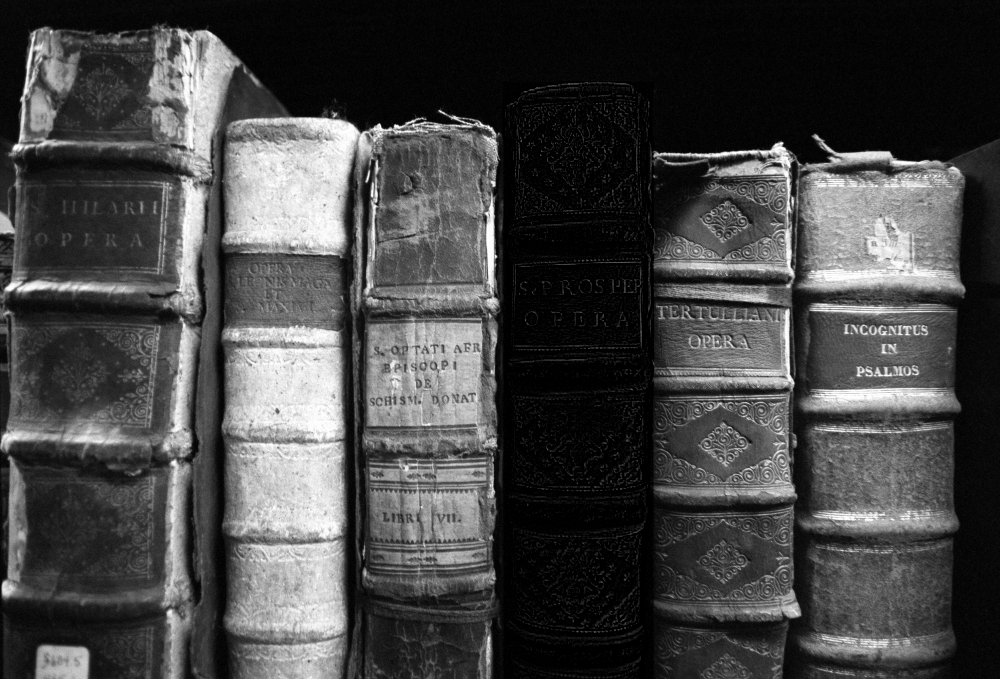
\includegraphics[scale=.2]{data/res/warped_bookT.png}}
\quad
\caption{Warped book subtracted from library}%
\label{fig:e2}%
\end{figure}

\section{SIFT in depth}
We have implemented our own version of SIFT. We have written methods to calculate custom Gauss pyramids with configurable sigma barriers and step sizes.
Then we subtracted these images pairwise to obtain a difference of gaussian pyramid.
In each of these images, we found the maximum absolute value and declared its location as a key point. The resulting key points can be seen in Fig. \ref{fig:e3}.
The problem is that we are only looking for global maxima. But when looking for local maxima, one would probably need to do some sort of non-maxima suppression or the result
will likely be even worse. Our interest points, even if not as many in numbers, are quite good, especially the ones on the book covers.

\begin{figure}%
\subfloat[][]{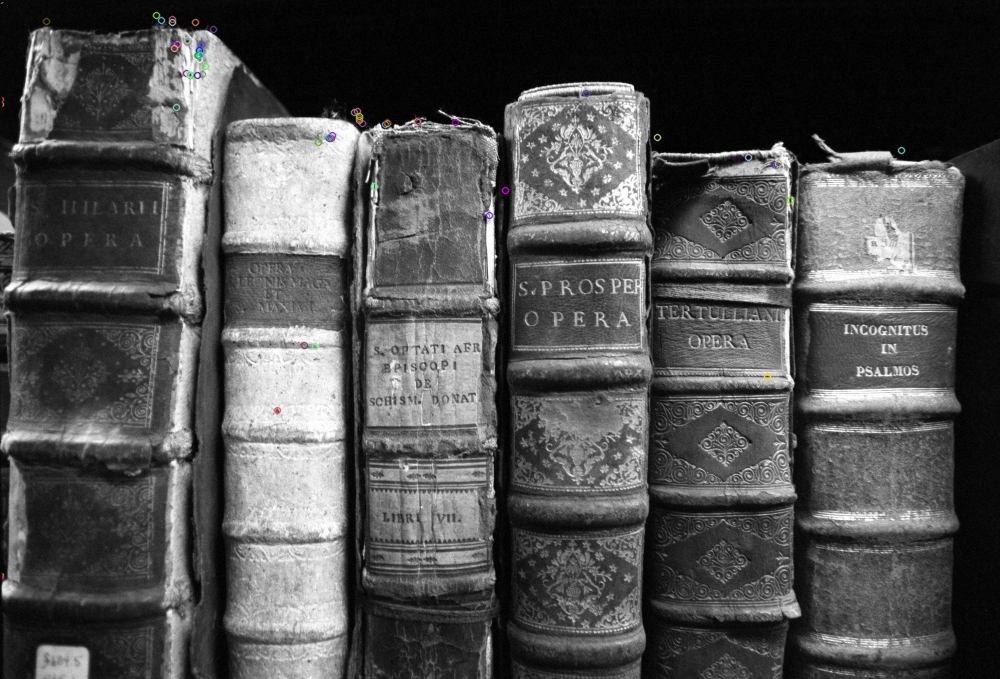
\includegraphics[scale=.4]{data/res/easysift.png}}
\caption{Keypoints detected by our SIFT implementation}%
\label{fig:e3}%
\end{figure}



\end{document}

